\section{Planteamiento del Problema}

Esta sección comprende el problema fundamental  y esencial para el desarrollo del plan de negocio propuesto, abordando las causas que establecen las necesidades de la creación del plan en cuestión con centro en el desperdicio de alimentos en las tiendas de barrio y plazas de mercado, así como el análsis de los distintos efectos que indican el impacto social y económico, lo anterior se puede ver representado en la \textit{Figura 1\ref{ArboldeProblema}}

\vspace{5mm}
\begin{minipage}{0.9\textwidth}
\centering
\label{ArboldeProblema}
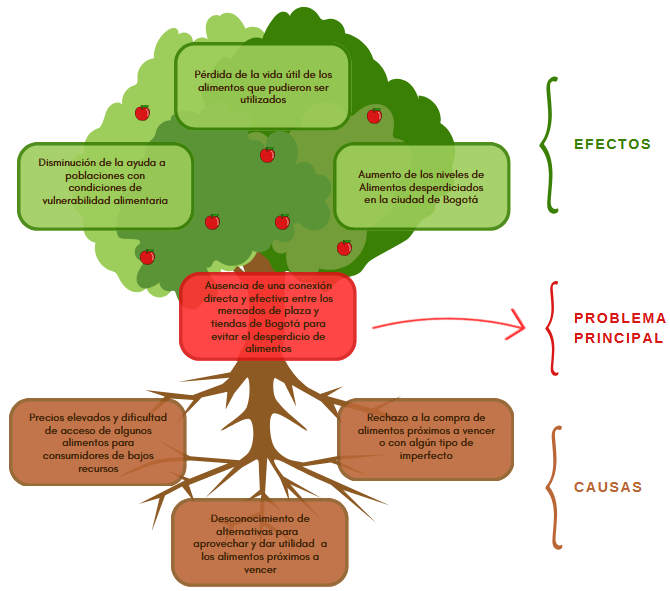
\includegraphics[width=0.7\textwidth]{Images/ArboldeProblema.png}
  %esto es lo nuevo que agregue
%\fnote{Nota. \textup{Fuente: \cite{documento_guia}}}
\end{minipage}
\textit{\captionof{figure}[{Árbol de problemas}]{ Árbol de problemas. Fuente: Elaboración propia. Adaptación (Rosario2020) }}



\import{./}{Content/2.PlanteamientoDelProblema/DescripcionDelProblema}
\import{./}{Content/2.PlanteamientoDelProblema/FormulacionDelProblema}
\import{./}{Content/2.PlanteamientoDelProblema/JustificacionDelProblema}